\chapter{Aufbau und Architektur von Blockchains}
\section{Begriffsdefinition}
Distributed ledger Technologie: Allgemeine Technologien, die ein verteiltes Hauptbuch beschreiben (Kerntechnologie der Blockchain) \textit{Vgl. \cite{Geiling.2016}}
Gelegentlich kommt in der Literatur der Begriff Distributed ledger vor. Dieser eignet sich sehr gut um das Kernprinzip von Crypto-Währungen zu beschreiben: Die dezentrale Speicherung sämtlicher im Netzwerk stattgefundener Transaktionen bei allen Teilnehmern im Netzwerk. Trotzdem ist der Begriff irreführend, da auf einer Blockchain kein klassisches Hauptbuch gespeichert wird, sondern lediglich eine Transaktionshistorie, aus der ein Hauptbuch mittels spezialisierter Software (i.d.R. \glqq Wallet\grqq{}-Programme) gebildet werden kann. Weiterhin gibt es Konzepte wie MaidSafe, die keine wie in Bitcoin verwendete Blockchain benutzen\footnote{http://blog.maidsafe.net/2016/01/10/evolving-terminology-pt-2/}. In dieser Arbeit werden nur Ansätze für smarte Verträge auf der Basis einer Blockchain betrachtet, d.h. ein Header, unter welchem alle Transaktionen gespeichert werden.
\section{Crypto-Währungen als digitales Zahlungsmittel}\todo{entscheiden, ob notwendig}
\section{Smarte Verträge}
\subsection{Begriffsdefinition}
Smarte Verträge werden derzeit sehr unterschiedlich definiert. Dies liegt wohl zum Großteil an einem unterschiedlichen Verständnis von Vertragsrecht über verschiedene Rechtssysteme hinweg - insbesondere zwischen dem in vielen Teilen der Welt praktizierten \glqq Common Law\grqq{} gegenüber dem in Kontinentaleuropa ausgeübten \glqq Civil Law\grqq{}, bzw. Zivilrecht. Doch auch verschiedene wissenschaftliche Disziplinen haben verschiedene Betrachtungsweisen - insbesondere Informatiker und Juristen haben hier unterschiedliche Einordnungen. Zusätzlich wirkt der Begriff smarter Vertrag irreführend. Er suggeriert, dass es sich bei einem smarten Vertrag um einen rechtlichen Vertrag handelt, der zusätzlich noch \glqq smart\grqq{} ist. Diese Arbeit zeigt, dass die Definition eines smarten Vertrags für sich selbst steht und dabei nicht der Definition eines rechtlichen Vertrags entsprechen muss.\\
Es wird sich an dem deutschen Vertragsbegriff orientiert, welcher insbesondere den Grundsatz der Privatautonomie beinhaltet. Eine allgemeingültige, globale Abgrenzung smarter Verträge zu rechtlichen Verträgen ist nicht Kern dieser Arbeit und wird an dieser Stelle nicht gesucht. Stattdessen wird eine pragmatische Definition im Kontext zu deutschem Vertragsrecht aufgezeigt, die es erlaubt, die in Kapitel \ref{chapter_anwendungsmöglichkeiten} aufgeführten Anwendungsmöglichkeiten smarter Verträge zu anderen Anwendungsmöglichkeiten, die nicht dieser Definition entsprechen, abzugrenzen.\\

Als Wortschöpfer gilt gemeinhin der Jurist und Informatiker Nick Szabo, welcher einen smarten Vertrag als \textit{\glqq eine Menge an Versprechungen, spezifiziert in digitaler Form, Protokolle beinhaltend, innerhalb welcher die Vertragsparteien ihre Versprechungen ausführen\grqq{}}, bezeichnet. \textit{\cite{Szabo.1996}}\\ \todo{Nees fragen ob Zitat übersetzt werden muss oder nicht}

Interessant ist hier, dass Szabo einen smarten Vertrag so definiert, dass er komplett innerhalb der spezifizierten Protokolle ausgeführt wird. Er ist also selbst-erfüllend. Damit grenzt er sich deutlich von den gängigen Vertragsdefinitionen ab, \todo{Überarbeiten} deren Erfüllung durch ein zugrundeliegendes Rechtssystem erzwungen werden kann. Diese Definitionen werden im folgenden betrachtet.\\

Nach dem \ac{BGB} definiert sich ein Vertrag wie folgt:\\
\textit{\glqq 
	Der Vertrag ist ein Rechtsgeschäft. Es besteht aus inhaltlich übereinstimmenden, mit Bezug aufeinander abgegebenen Willenserklärungen (Angebot und Annahme) von mindestens zwei Personen.\\
	Durch den Grundsatz der Vertragsfreiheit (Privatautonomie) wird sichergestellt, dass jeder Mensch das Recht hat, im Rahmen der Gesetze seine Verhältnisse durch Verträge eigenverantwortlich zu gestalten.\grqq{}}
\todo{Zitat}\\

Einen rechtlichen Vertrag definiert Szabo als:
\textit{\glqq  eine Menge an Versprechungen welche in einer \glqq Übereinstimmung gegenseitiger Vorstellungen\grqq{} getroffen werden.\grqq{}}\\


Ein großer Unterschied beider Definitionen besteht sowohl in der Vertragsausgestaltung als auch in der Definition der Vertragspartner. Laut BGB ist ein Vertrag ein Rechtsgeschäft. Dies setzt unter anderem voraus, dass beide Vertragspartner geschäftsfähig sind.\footnote{https://de.wikipedia.org/wiki/Rechtsgesch\%C3\%A4ft} \todo{Quelle}
Geschäftsfähig können entweder juristische oder natürliche Personen sein. \footnote{http://www.steuerazubi.com/geschaeftsfaehig} \todo{quelle}
Ein Vertrag zwischen Entitäten, die nicht dieser Definition entsprechen, kann somit aus rechtlicher Sicht nicht Zustandekommen.\\

Bezüglich der Vertragsgestaltung setzt das BGB die Einschränkung, dass ein Vertrag nur im Rahmen der Gesetze gestaltet werden kann. Im Rahmen des BGB gilt entsprechend deutsches Recht. Dies umfasst beispielsweise die Essentialia negotii\footnote{https://en.wikipedia.org/wiki/Essentialia\_negotii}, die minimalen Inhalte, welche ein Vertrag benötigt um rechtlich bindend zu sein, oder vom Gesetzgeber geforderte Vertragsformen. Eine exakte Aufstellung wird an dieser Stelle nicht vorgenommen.\\

Durch den nicht vorhandenen Rechtsraum in welchem smarte Verträge auf der Blockchain ausgeführt werden,\footnote{Durch pseudonyme Vertragspartner sowie die globale Verteilung der Nodes ist eine Zurückverfolgung der Vertragsparteien auf einen spezifischen Rechtsraum nicht möglich.} kann auch kein lokales Recht aufgeführt werden. Die Vertragsdefinition soll laut Szabo in digitaler Form, d.h. in maschinenlesbarem Code vorgenommen werden.
 Auch die Vertragsparteien unterliegen nach der Definition Szabos keiner Einschränkung. \\
 Als Besonderheit smarter Verträge auf der Blockchain gilt, dass die beiden Parteien sich durch die Pseudonymisierung ihrer Accounts nicht kennen, wodurch der smarte Vertrag mit dem auf der Blockchain installiertem Computerprogramm getroffen wird, welcher selbst den Vertrag darstellt. Als Beispiel dient das in Abschnitt \todo{Abschnitt angeben} beschriebene Forward-Rate-Agreement.\\

\todo{macht vermutlich am Ende mehr Sinn}Zusammenfassend wird für smarte Verträge auf der Blockchain folgende Definition getroffen:\\
\textit{\glqq Smarte Verträge sind auf der Blockchain installierte Programme, welche von den Vertragspartnern, oder anderen smarten Verträgen aufgerufen werden. Die Vertragsbedingungen bestehen aus in maschinenlesbarem Code definierten wenn-dann Bedingungen. Ihre Erfüllung wird ex-ante durch den Code erzwungen.\grqq{}}\todo{Auch ein Vertragsbruch im Sinne von: Ich muss aus dem Vertrag aussteigen, deshalb bezahle ich vorab eine Kaution, die ich dafür bezahlen muss, wäre eine erzwungene Vertragserfüllung.}

\subsection{Einführung}

Der Begriff der smarten Verträge wurde bereits 1995 von Nick Szabo definiert und damit einige Zeit vor der ersten Beschreibung der Blockchain-Technologie. Sein Ziel ist es, verschiedene Aspekte von Verträgen so in Hardware und Software einzubinden, dass ein Vertragsbruch entweder teuer oder unmöglich für den Vertragsbrecher wird. \\
Als Beispiel für einen \glqq Urahnen\grqq{} eines smarten Vertrags führt er den Verkaufsautomaten auf. Juristisch gesehen wird mit den angegeben Produktpreisen ein Angebot abgegeben, dem ein Käufer durch Einwerfen einer passenden Summe zustimmt. Der Verkaufsautomat kommt darauf durch Ausgabe des Produkts seiner juristischen Bringschuld nach. Für den Käufer ist ein Vertragsbruch prinzipiell nicht möglich, da er verpflichtet ist, den passenden Geldbetrag zu zahlen, bevor das Produkt ausgegeben wird. Für den Automaten ist er unmöglich, da aufgrund des einprogrammierten Vertrags das passende Produkt nach Bezahlung ausgegeben wird. %Während beim Verkaufsautomat der hinterlegte Code nicht einsehbar ist, sollte dies nicht für smarte Verträge gelten. 
\textit{\cite{Szabo.1997}} \\

Verträge müssen nach Szabo folgende Design-Prinzipien erfüllen:
\begin{labeling}{vertrauliches Mitwissen}
	\item[Beobachtbarkeit] Es muss für beide Parteien der Fortschritt der Vertragserfüllung der anderen Partei beobachtbar sein, oder es muss Möglich sein, den Fortschritt gegenüber anderen Klienten zu beweisen.
	\item[Überprüfbarkeit] Es muss für einen Klienten möglich sein, einem Schlichter gegenüber zu beweisen, ob ein Vertrag gebrochen oder eingehalten wurde.
	\item[vertrauliches Mitwissen] Wissen und Kontrolle über die Vertragsinhalte und die Vertragserfüllung sollten an die verschiedenen Parteien nur so weit verteilt werden, wie es für die Vertragserfüllung notwendig ist.
	\item[Durchsetzbarkeit] Durchsetzbarkeit beschreibt sowohl die Möglichkeit, dass ein smarter Vertrag so aufgebaut ist, dass er seine Einhaltung selbst erzwingt, als auch dass durch die Überprüfbarkeit eine dritte Partei eine Ausführung erzwingen kann.
\end{labeling}
\textit{\cite{Szabo.1996}}

Ähnliche Design-Prinzipien sollen auch für die Definition smarter Verträge gelten. 

\subsection{Anwendung auf der Blockchain}
Typischerweise erfüllt ein smarter Vertrag auf der Blockchain folgende Funktionen:
\begin{enumerate}
	\item Es wird der smarte Vertrag als Code definiert.
	\item Dieser Code wird durch Implementierung in ein verteiltes Netzwerk in Produktion gesetzt.
	\item Partei eins steigt in den Vertrag ein, indem sie einen gewissen Token zu einer von dem Code kontrollierten Adresse sendet.
	\item Zusätzliche Parteien steigen in den Vertrag mit dem selben Mechanismus ein.
	\item Sobald ein Ereignis eintritt, welches den Code auslöst, werden verschiedene Funktionen ausgeführt, die voraussichtlich die Tokens neu zwischen den teilnehmenden Parteien verteilt.
\end{enumerate}
\textit{\cite{Valkenburgh.2015}}

Um eine Übereinstimmung der Willenserklärungen zu gewährleisten, muss der Code für die Partei, die den smarten Vertrag ausführt ersichtlich sein. Dies kann bei einem an alle Nutzer gerichteten smarten Vertrags durch eine Veröffentlichung des Codes geschehen. Dies widerspricht jedoch dem Design-Prinzip des vertraulichen Mitwissens. \todo{Problem, bzw. Lösung erläutern}
Überprüfbar sind die Vertragsbedingungen beispielsweise über den kompilierten Code des smarten Vertrags und/oder mittels eines Hashwerts. 
Tokens können 

\begin{figure}[ht]
	\centering
	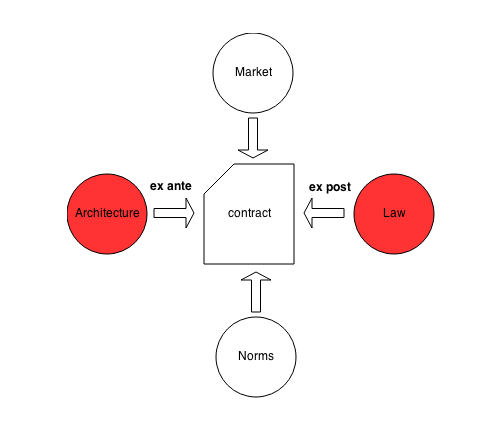
\includegraphics[scale=0.75]{grafiken/smart_contract_time_dimension.png}
	\caption{Smart Contracts im zeitlichen Kontext.  \textit{Vgl. \cite{Glatz.2014}}}
	\label{smart_contracts_time_dimension}
\end{figure}


Ein smarter Vertrag muss dabei nicht zwingend einem juristischen Vertrag entsprechen.\todo{ausführen}\\

 Dabei haben sie einen entscheidenden Unterschied gegenüber juristischen Verträgen: die zeitliche Komponente. Während 
\section{Entwurf der Blockchain nach Satoshi Nakamoto}
\subsection{Der Header}


Für die Entwicklung der Technologie hinter Bitcoin wurden verschiedene bekannte Techniken aus den Bereichen Kryptographie, verteilte Systeme, Datenstrukturen miteinander verknüpft. Den zentralen Teil stellt eine verkettete Liste dar, die in jedem Node - jedem Teilnehmer in dem Netzwerk - gespeichert wird. Jeder Listeneintrag beinhaltet einen Header mit Metadaten, der im folgenden beschrieben wird. Weiterhin enthält er eine genaue Auflistung aller in diesem Eintrag zusammengefassten Transaktionen. Ein header mit allen enthaltenen Transaktionen wird Block genannt. Da ein Block immer auf seinen Vorgänger verweist, entsteht eine Verkettung aller Blöcke untereinander, wodurch der Name Blockchain entstanden ist.\\

\begin{lstlisting}[language=html, caption=Ein beispielhafter Block-Header \cite{Webbtc.2015} \label{Beispiel_Block}]
{
"hash": "000000000000000001f942eb4bfa0aeccb6a1...",
"ver": 2,
"prev_block": "00000000000000000a3ed9a4e2540751...",
"mrkl_root": "9b7d5896398581a7ff26be4b3684ddd95a...",
"time": 1432723472
"bits": 404129525,
"nonce": 226994584,
"n_tx": 1031,
"size": 749157,
"tx": [
{...
}]
}
\end{lstlisting}

Der Block-Header, wie beispielhaft in Liste \ref{Beispiel_Block} angegeben, beinhaltet folgende Elemente:\\


\begin{labeling}{prev\_block}
	\item[hash] ein Hash des kompletten Headers
	\item[ver] Eine Versionsnummer, die Software/Protokoll-Upgrades anzeigt
	\item[prev\_block] Der previous\_block ist die Referenz auf den vorherigen Block. Dadurch kann jede getätigte Transaktion bis zum ersten Block, dem sogenannten Genesis-Block zurückgeführt werden
	\item[mrkl\_root] Die Merkle Root ist ein Hash sämtlicher Transaktionshashes, wodurch sich alle Transaktionen effizient zusammenfassen lassen. Das genaue Vorgehen sowie der Einsatzzweck sind in Abschnitt \todo{Referenz}beschrieben
	\item[time] Ein Zeitstempel des Blocks
	\item[bits] Die angestrebte Schwierigkeit der Berechnung des Blocks
	\item[nonce] Eine Zufallszahl. Sie ist die Zahl, mit welcher der Hash des Blocks errechnet wird. Ein Miner probiert dazu verschiedene Zufallszahlen aus, bis er auf die gesuchte oder eine höherwertige gestoßen ist.
	\item[n\_tx] Die Anzahl der im Block enthaltenen Transaktionen
	\item[size] Die Größe des Blocks in Bytes
	\item[tx] Die durchgeführten Transaktionen in Listenform
\end{labeling}
\textit{Vgl. \citet{Antonopoulos.2015}, S.161}

Es ist anzumerken, dass im eigentlichen JSON-Format eines Blocks kein Eintrag gegeben ist, an welcher Position nach dem Genesis-Block ein spezifischer Block steht. Dieser Wert wird oft angegeben zur einfachen Identifizierung eines Blocks, ist jedoch nicht immer eindeutig, da im Fall einer Gabelung der Chain zwei Blöcke die gleiche Positionsnummer haben können.

\subsection{Transaktionen}
\todo{Eventuell Schlüsselaustausch beschreiben?}
\subsubsection{Vorgehen}
Um Transaktionen durchzuführen, wird ein gültiger privater sowie öffentlicher Schlüssel benötigt. Dieser kann selbst erzeugt werden, z.B. durch die Installation eines Wallets, oder von einem externen Dienstleister wie einer Börse, welche die Schlüssel sowie das Guthaben verwaltet. Das Schlüsselpaar wird per ECDSA-Verfahren erzeugt, wobei der öffentliche Schlüssel danach weitere Hashfunktionen durchläuft, so dass eine Berechnung des privaten Schlüssels aus dem öffentlichen mit extrem hohen Aufwänden verbunden ist. \\
Umgekehrt lässt sich der öffentliche Schlüssel jedoch relativ einfach aus dem privaten Schlüssel generieren, wodurch es für einen Angreifer genügt, in Besitz des privaten Schlüssels zu kommen um ein Wallet komplett in seinen Besitz zu bringen. Theoretisch ist ein zufälliges Erraten eines privaten Schlüssels sehr unwahrscheinlich, da es für den 32-Byte langen Schlüssel 10\textsuperscript{77} Kombinationsmöglichkeiten gibt. \textit{Vgl. \cite{Antonopoulos.2015}} \todo{Seitenzahl angeben}
Zum Vergleich: Es wird geschätzt, dass es 10\textsuperscript{78} Atome im Universum gibt. Zufällig einen privaten Schlüssel zu finden, der auf ein gültiges Konto mit Guthaben referenziert, ist also extrem unwahrscheinlich. \textit{Vgl. \citet{UniversitatFrankfurt.2016}}\\


\begin{figure}[ht]
	\centering
	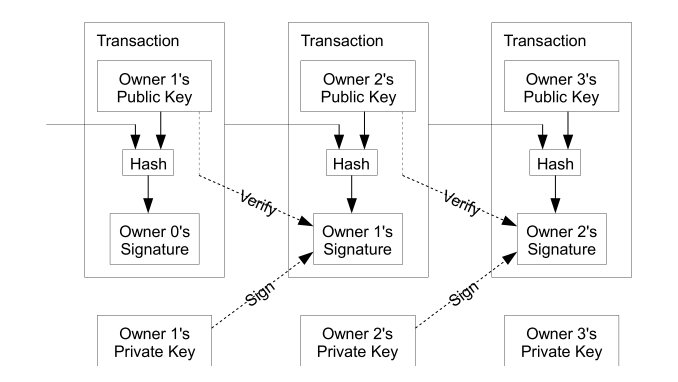
\includegraphics[scale=0.75]{grafiken/Blockchain_Transaktionen.png}
	\caption{Die Transaktionskette Vgl. \citet{Nakamoto.2008}, S.2}
	\label{Transaktionskette}
\end{figure}

Ein bis zur Entwicklung des Bitcoin-Protokolls nicht gelöstes Problem, war die Möglichkeit des \glqq double-spending\grqq{} von Crypto-Währungen. Bei diesem Verfahren wird eine Geldeinheit and 2-n Empfänger überwiesen. Erhalten diese die Transaktionsnachricht gleichzeitig wird festgestellt, dass der Wert dem Sender noch nicht abgebucht wurde und Werten die Transaktion somit als gültig. Bisher wurde eine zentrale Instanz benötigt, die validiert hat, dass ein Wert nicht bereits an einen anderen Empfänger überwiesen wurde. Abbildung \ref{Transaktionskette} zeigt, wie sich dieses Problem dezentral lösen lässt. Will B einen Betrag an C überweisen \todo{Satoshis Zeichnung anpassen}, muss C sicherstellen können, dass 
\begin{enumerate}
	\item B der Betrag gehört
	\item B den Betrag nicht schon an jemand anderen überwiesen hat
\end{enumerate}

Dazu wird die vorherige Transaktion A --> B zusammen mit dem Public Key von C gehasht und schließlich mit B's privatem Schlüssel verschlüsselt \todo{Besseres Wort}. 
C kann nun die Transaktion mit dem öffentlichen Schlüssel von B entschlüsseln und erhält den von B zuvor generierten Hashwert. C kann diesen nun selbst generieren und weiß bei Übereinstimmung, dass kein Betrugsfall vorliegt. Dadurch ergibt sich eine Transaktionskette bis zum ersten \glqq prägen\grqq{} des Betrags, der sogenannten Coinbase-Transaktion. Diese wird automatisch als Belohnung für das Lösen neuer Blöcke - dem sogenannten Minen - ausgezahlt, wodurch neue Münzen in den Bitcoin-Kreislauf gelangen.\\

Guthaben werden nicht klassisch in einer Datenbank gespeichert, sondern sind in der Blockchain als \ac{UTXO} einer Adresse zugeordnet. Wenn eine Wallet-Software also die Bilanz eines Kontos errechnet, werden alle Transaktionen die dem Besitzer des Wallets zugeordnet sind, ermittelt und diejenigen, die noch nicht übertragen worden sind, aufsummiert. 
eine \ac{UTXO} ist unteilbar, d.h. Überweisungen werden aus \ac{UTXO}'s zusammengesetzt. Ist dieser Input höher als der sich daraus ergebende Output an die neue Adresse, wird die Differenz (abzüglich einer Transaktionsgebühr) als neuer \ac{UTXO} an den Sender als Wechselgeld zurücküberwiesen. \cite{Antonopoulos.2015}[S.112ff]

\begin{figure}[ht]
	\centering
	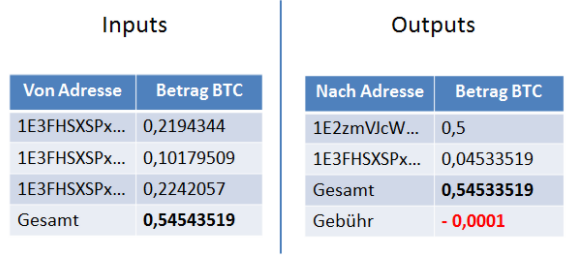
\includegraphics[scale=0.75]{grafiken/transaktion_input_output.png}
	\caption{Input und Output einer Transaktion }
	\label{input_output}
\end{figure}
\todo{eigene Zeichnung}
Abbildung 2.2 stellt eine Transaktion dar. Um eine Überweisung von 0,5 \ac{BTC} werden \ac{UTXO} im Wert von mindestens 0,5 \ac{BTC} der Adresse 1E3FHSXSPx... gesammelt. Sind diese gefunden, wird der Betrag von 0,5 \ac{BTC} an die Zieladresse 1E2zmVJcW... gesendet. Die Differenz - abzüglich einer Gebühr von 0,0001 \ac{BTC} - wird als neue \ac{UTXO} an den Empfänger zurücküberwiesen.

\subsubsection{Transaktionsarten}
Im Bitcoin-Protokoll sind neben der standardmäßigen Überweisung an eine öffentliche Adresse noch weitere Transaktionsarten für andere Einsatzzwecke möglich: 

\begin{labeling}{Multi Signature}
	\item[P2PKH] Der Pay-to-Public-Key-Hash ist das, was bei Bitcoin als die normale Überweisung an einen Empfänger gilt. Der Hash des öffentlichen Schlüssel des Empfängers stellt dabei dessen Adresse dar.
	\item[PTPK] Die Pay-to-Public-Key Variante ist eine vereinfachte Form des PTPKH, bei dem direkt an den öffentlichen Schlüssel gezahlt wird. Dies wurde zu Beginn von Bitcoin für Coinbase-Transaktionen genutzt, ist jedoch mittlerweile veraltet.
	\item[Multi Signature] Das Multi Signature Verfahren speichert N öffentliche Schlüssel im Skript, von denen eine Teilmenge M die Transaktion bewilligen muss, um diese auszulösen.
	\item[Data Output] Das Data Output Feld, bzw. op\_return Feld erlaubt es zusätzliche Informationen an eine Transaktion einzufügen, z.B. den digitalen Fingerabdruck einer Datei, die folgenden Vertrag darstellt: \glqq Ich erkläre hiermit, die Wertanlage A an XYZ zu Zeitpunkt ZEITSTEMPEL zu übergeben!\grqq{} Eine solche Transaktion kann nicht mehr weitergeleitet werden - sie kann nur einmal genutzt werden. Werden mit ihr Bitcoins übertragen, so sind diese Verloren, da sie nicht mehr ausgegeben werden können. \todo{Vermutlich wird dies für den Proof-of-Burn ansatz genutzt} In der Bitcoin-Community werden solche Übertragungen zwiespältig angesehen, da sie nicht die grundlegenden Funktionen der Übertragung von Bitcoins nutzen, andererseits aber zeigen, welche Anwendungsmöglichkeiten eine sichere und schwer manipulierbare Blockchain bietet. Aus diesen Gründen ist das op\_return Feld auf 40 byte limitiert. 
	\item[P2SH] Bitcoin verwendet zur Validierung von Transaktionen eine Skript-Sprache. Diese ist in ihrer Funktionalität sehr eingeschränkt, beispielsweise können keine Schleifen programmiert werden. Diese Einschränkung soll ein zuspammen des Netzwerks durch Funktionen mit Endlosschleifen oder anderen unlösbaren Rechnungen verhindern. Dennoch lassen sich Skripte mit einer gewissen Komplexität erzeugen, wie beispielsweise das Multi Signature Verfahren. Bei dem Pay-to-Script-Hash Verfahren wird der Hash des Skripts als Adresse verwendet und erst nach Validierung der Hashwerts das Skript ausgeführt. Dadurch werden Transaktionen insbesondere für Sender einfacher, da sie nur den Hashwert des Skripts brauchen und das eigentliche Skript verborgen werden kann.
\end{labeling}
\textit{\cite{Antonopoulos.2015}, S.127ff}
\subsection{Peer-to-peer Netzwerke}

Das Bitcoin Netzwerk ist als sogenanntes peer-to-peer Netzwerk aufgebaut. Es folgt dabei einer Architektur, die nicht dem zentralen Client/Server Aufbau entspricht, in welchem ein, bzw. mehrere zentrale Server die Anfragen von Clients bearbeiten. Stattdessen ist jeder Peer gleichzeitig Client und Server, wodurch es keinen zentralen Single-Point-of-failure gibt. Ein Beispiel für ein bekanntes peer-to-peer Netzwerk ist Bittorrent, als Netzwerk zum Filesharing. Dennoch können Nodes verschiedene Anwendungszwecke haben und somit unterschiedliche Aufgaben erfüllen:

\begin{labeling}{Kompletter Blockchain Node}
	\item[Referenz Client] enthält Wallet, Miner, die komplette Blockchain und einen Network Routing Node
	\item[Kompletter Blockchain Node] Enthält die komplette Blockchain und einen Network Routing Node
	\item[Solo Miner] Enthält einen Miner, die komplette Blockchain und einen Network Routing Node
	\item[SPV-Wallet] Ein \ac{SPV}-Wallet Enthält ein Wallet und einen Network Node
	\item[Pool mining Node] Enthält einen Miner und einen Network Routing Node der auf einen Mining Pool zugreift
\end{labeling}
\textit{\cite{Antonopoulos.2015}, S.140}\\
Ein Wallet stellt die digitale Geldbörse dar, in der Schlüsselpaare sowie Adressen der Nutzer gespeichert sind. Oft haben Wallets zusätzliche Funktionalitäten wie die Berechnung der Bilanz oder Verschlüsselung des Wallets zur Erhöhung der Sicherheit.\\
Ein Miner ist ein Programm, dass genutzt wird um die mathematischen Rätsel der Blockchain zu lösen. Ein Solo Miner benötigt dazu eine komplette Kopie der Blockchain, während einem Miner in einem Mining Pool i.d.R. ein Teil zur Berechnung zugewiesen wird.\\
Die komplette Blockchain beinhaltet alle Blockheader sowie deren Transaktionen. Bei anderen Nodes werden nur die Header gespeichert.\\
Der Network Routing Node beinhaltet alle Funktionalitäten, die zur Kommunikation mit den anderen Nodes im Netzwerk benötigt werden.

\subsection{Aufbau und Lösen von Blöcken}
\subsubsection{Mining}
Als Mining wird das Lösen von Blöcken bezeichnet. Jeder Block ist mit einem mathematischen Rätsel versehen, das gelöst werden muss, damit ein Block in die Blockchain aufgenommen wird. dabei wird ein Rätsel benötigt, welches folgende Attribute aufweist: 
\begin{enumerate}
	\item Schwer zu errechnen
	\item Leicht zu validieren
	\item Einfach zu skalieren
\end{enumerate}
Die Skalierbarkeit wird benötigt um die Berechnungszeit konstant zu halten. Bei zu geringen Berechnungszeiten entstehen viele Side-Chains und die Wahrscheinlichkeit, dass eine Instanz für einen gewissen Zeitraum genügend Blöcke löst um das System zu manipulieren, steigt stark an. Bei zu hohen Berechnungszeiten dauern Transaktionen sehr lange und das System wird ineffektiv. Die angestrebte Blockbildungszeit beträgt bei Bitcoin 10 Minuten, bei den meisten anderen Währungen liegt sie zwischen 1-10 Minuten. \cite{Pfnur.2014}[S.36]\\

Bitcoin verwendet als Rätsel den SHA256 Algorithmus. Der \glqq hash\grqq{} Eintrag eines Block-headers hasht den kompletten Header. In Liste \ref{Beispiel_Block} sieht man, dass dieser Hash mit einer gewissen Anzahl nullen beginnt. Diese stellen die Schwierigkeit der Berechnung dar und werden über den Wert \glqq nonce\grqq{} gelöst. Wird ein neuer Block gebildet, so ist der Wert der Nonce auf 0. Die über das Feld \glqq bits\grqq{} angegebene Schwierigkeit sagt aus, mit wie vielen Nullen der Hash beginnen muss, damit der Block als gelöst gilt. Ein Miner hat zur Berechnung keine andere Möglichkeit als so lange Werte für die Nonce auszuprobieren, bis er auf das korrekte Ergebnis stößt. Dieses Ergebnis wird von dem Miner über das Netzwerk publiziert. Andere Nodes können den Hashwert des neuen Blocks durch die Hashfunktion mit der berechneten Nonce einfach validieren, wodurch sich ein gemeinsamer Konsens auf den neuen Block bildet. Bei ausreichendem Konsens wird der Miner belohnt und die Transaktionen werden ausgeführt. Da für dieses Verfahren Rechenleistung und Strom der Miner aufgewendet werden, die Rechner also für die Lösung \glqq arbeiten\grqq{}, wird dieses Verfahren Proof-of-Work genannt. \cite{Nakamoto.31.10.2008}[S.3] \\
 
\subsubsection{Belohnungen für das Mining}
Die Belohnung für den Miner besteht in der Auszahlung einer gewissen Anzahl Bitcoins, die als erste Transaktion des neuen Blocks ausgeführt wird. Diese wird als Coinbase Transaktion bezeichnet, da sie als einzige keine einem Sender zugehörige Adresse hat, sondern die Bitcoins neu erzeugt werden. Zusätzlich erhält der Miner alle anfallenden Transaktionsgebühren. Transaktionsgebühren sind vom Sender festgelegte Gebühren, die ihm eine höhere Priorität bei der Aufnahme in Blöcke verschaffen. Blocks haben eine maximale Größe.\footnote{https://en.bitcoin.it/wiki/Block\_size\_limit\_controversy}
Transaktionen werden nach absteigender Priorität Blöcken nach folgender Formel hinzugefügt:\\
\begin{center}
	$priority = \sum\nolimits_{n=0}^N \frac{Wert\ des\ Inputs\ *\ Alter\ des\ Inputs}{Groesse\ in\ Bytes}$
\end{center}


	Mit zunehmendem Alter steigt also die Priorität, eine Transaktion dem Block hinzuzufügen, selbst wenn keine Transaktionsgebühren bezahlt wurden. Da die Anzahl über die Coinbase-Transaktion ausgezahlter Bitcoins degressiv verläuft und auf 21. Mio Bitcoins limitiert ist, soll Zukünftig die Belohnung der Miner ausschließlich über Transaktionsgebühren erfolgen. \cite{Nakamoto.31.10.2008}[S.4]
	Ein solches Vorgehen hat einen zusätzlichen positiven Nebeneffekt: Es verhindert das \glqq zuspammen\grqq{} des Netzwerks mit wertlosen bzw. sehr geringwertigen Transaktionen, was einem \ac{DoS} Angriff gleichkäme.

\subsubsection{Duplizierte Chains}
Sollten zwei Miner zeitgleich einen Block lösen und über das Netzwerk propagieren, so werden beide zunächst als gültig erklärt und Miner arbeiten an jeweils dem Block, der sie zuerst erreicht hat. Sobald nun einer der beiden Blöcke gelöst wurde, arbeiten Miner an der längeren Chain, wodurch die kürzere nicht mehr bearbeitet wird und damit ungültig wird. In diesem ungültig gewordenen Block enthaltene Transaktionen werden wieder dem Pool an Transaktionen hinzugefügt und in den kommenden Blöcken verarbeitet. 
\subsection{Manipulationssicherheit}
\subsection{Der Einsatz von Merkle-Trees zur effizienten Validierung von Blöcken}
\subsubsection{Berechnung der Merkle-Root}
Mit Hilfe von Merkle-Trees lässt sich ein Block sehr effizient validieren. Die im Block-Header angegebene Merkle Root ist eine Zusammenfassung der Hashwerte aller Transaktionen.

\begin{figure}[ht]
	\centering
	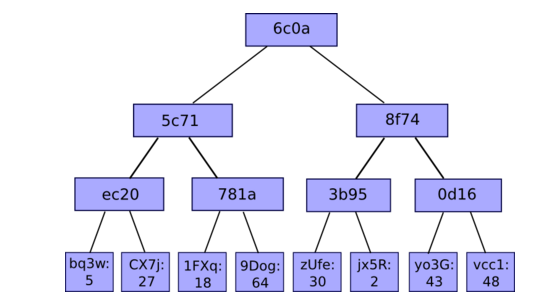
\includegraphics[scale=0.75]{grafiken/merkle_tree.png}
	\caption{Beispiel für einen Merkle Tree \cite{Buterin.2014}}
	\label{Beispiel für einen Merkle Tree}
\end{figure}\todo{Vernünftige Grafik einbauen}

Abbildung \ref{Beispiel für einen Merkle Tree} stellt Grafisch den Algorithmus dar. Die Blätter des Baums sind die Hashwerte der einzelnen Transaktionen. In diesem Fall werden acht Transaktionen angenommen. Der Merkle Tree fasst diese Transaktionen immer paarweise zusammen [0,1][2,3][4,5][6,7] und erstellt einen Hash aus diesen. Aufgrund seiner Struktur benötigt der Merkle Tree immer eine gerade Zahl an Transaktionen. Ist diese nicht gegeben, wird der letzte Hashwert verdoppelt um den Baum auszubalancieren. Im Falle des Bitcoin Protokolls wird zweimal mit dem SHA256 Algorithmus gehasht. Dieser Vorgang wird solange wiederholt, bis ein Hashwert übrigbleibt: Die Merkle Root.\\
Versucht nun ein Angreifer eine Transaktion \glqq einzuschmuggeln\grqq{}, ändert sich der Hashwert der Merkle-Root. Es kann also die Validität eines Blocks effizient überprüft werden, ohne jede Transaktion abzugleichen.\\
Dies ist eine Voraussetzung für das Betreiben von unvollständigen Nodes, die nur die Block-Header speichern. \cite{Nakamoto.31.10.2008}[S.5]

\subsubsection{Simplified Payment Verification durch Merkle-Path}
Die \ac{SPV} speichert nur die Block-Header. Dadurch ist diese Form von Node sehr leichtgewichtig und kann beispielsweise auch auf einem Smartphone betrieben werden. 

\begin{figure}[ht]
	\centering
	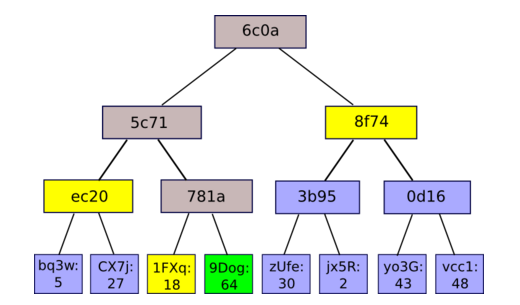
\includegraphics[scale=0.75]{grafiken/merkle_path.png}
	\caption{Beispiel für einen Merkle Path \cite{Buterin.2014}}
	\label{Beispiel für einen Merkle Path}
\end{figure}\todo{Vernünftige Grafik einbauen}

Um zu ermitteln ob ein Input einer Zahlung gültig ist, kann ein \ac{SPV} nicht alle Transaktionen durchgehen. Zur Autorisierung müssen daher Full Nodes angefragt werden. Dazu werden die benötigten Merkle Hashes zur Bildung eines Pfads zur eigentlichen Transaktion abgefragt. In Abbildung \ref{Beispiel für einen Merkle Path} wird Block 9Dog abgefragt. Zum verifizieren der merkle\_root werden nur noch Block ec20 und 8f74 benötigt. \cite{Buterin.2016}
\subsection{Mining Pools}
\section{Erweiterungen des Bitcoin-Protokolls}
\subsection{Arten von Chains}
\begin{table}[]
	\centering
	\caption{Arten von Blockchains}
	\label{chain-arten}
	\begin{tabular}{lll}
		\hline
		\textbf{Art der Chain} & \textbf{Art der Cryptowährung} & \textbf{Beispiele}                 \\ \hline
		Bitcoin Blockchain     & Bitcoin                        & Bitcoin                            \\
		Bitcoin Blockchain     & Altcoin                        & Counterparty                       \\
		Sidechain      & Bitcoin                        & Rootstock, Testversionen von Bitcoin  \\
		Sidechain      & Altcoin                        & Dogecoin, Ethereum, Litecoin, Dash \\ \hline
	\end{tabular}
\end{table}

Tabelle \ref{chain-arten} zeigt die verschiedenen existierenden Chain-Arten. Die meisten existierenden Coins basieren auf Klonen der Bitcoin Blockchain in denen einige Paramater geändert worden sind, wie z.B. der PoW-Algorithmus, die Blocklösungszeit, etc. Beispiele sind Dogecoin, Dash oder Litecoin. 

\subsection{Übertragung von Werten zwischen verschiedenen Chains}
\todo{Keine Erweiterung des Bitcoin-Protokolls sondern anwendbar auf alle chains}
Durch verschiedene Modelle lassen sich Werte zwischen verschiedenen Chains übertragen und auf diesen halten. %Bei Bitcoin lassen sich benötigte Erweiterungen als Soft-Fork realisieren.


\subsubsection{Gemeinsames Mining}
In den unten beschriebenen Konzepten wird die Bitcoin-Blockchain als Parent-Chain und mögliche andere Chains als Side-Chains bezeichnet. Sidechains können dabei entweder 
\begin{enumerate}
	\item Auf der Bitcoin-Blockchain aufsetzten und keine eigene Währung besitzen
	\item Auf der Bitcoin-Blockchain aufsetzten und 1-n eigene Währungen besitzen (Counterparty)
	\item Nicht auf der Bitcoin-Blockchain aufsetzen
\end{enumerate}

Dabei liegt die Annahme zugrunde, dass eine Sidechain die Möglichkeit bieten möchte, Transaktionen innerhalb der Chain mit Bitcoin ausführbar zu machen, da Bitcoin als Währung mit der höchsten Marktkapitalisierung am bekanntesten ist und am häufigsten benutzt, kann so die Einstiegshürde gesenkt werden. \\
Eine weitere Annahme ist, dass die Sidechain bereit ist, ihr Protokoll so anzupassen, dass auf ihr entweder nur, oder zusätlich noch Bitcoin gehandelt werden kann. Zur Realisierung im Bitcoin-Protokoll soll jedoch maximal ein Soft-Fork möglich sein, d.h. eine abwärtskompatible Anpassung, in der es für Miner, die ihr Protokoll nicht updaten, keine Einschränkungen gibt.
\subsubsection{One-way peg}
Der One-way peg erlaubt den Transfer von Einheiten in eine Richtung.\footnote{https://www.mail-archive.com/bitcoin-development@lists.sourceforge.net/msg02346.html} Dazu wird eine Geldeinheit an eine nicht weiterverwendbare Adresse geschickt. Durch den Nachweis, dass die Transaktion stattgefunden hat, sowie einem Nachweis, dass man der Sender der Transaktion war (i.d.R. über den Private-Key), werden einem auf einer anderen Chain eine entsprechende Menge an Geldeinheiten über eine Coinbase-Transaktion gutgeschrieben. Diese Methode ist vergleichsweise einfach implementierbar und relativ sicher. Jedoch kann sie nur in eine Richtung verwendet werden, da die gesendete Geldeinheit nachweisbar zerstört werden muss. Der Ansatz entspricht dem Proof-of-burn Ansatz.\\ 
Erstmals wurde er von der Firma Counterparty verwendet.\todo{Zitat	} Sie bietet erweiterte Funktionalitäten auf der Bitcoin-Blockchain wie z.B. dem Erstellen eigener Tokens. Dafür besitzt sie eine eigene Währung (XCP), welche durch \glqq verbrennen\grqq{} von Bitcoins erstellt worden ist. Transaktionen in XCP werden über eine Gebühr in Bitcoins bezahlt, wodurch Bitcoin-Miner einen Anreiz haben, XCP-Transaktionen in Bitcoin-Blöcken aufzunehmen.
\subsubsection{Symmetrischer two-way peg}
Beim two-way peg wird statt einer nicht mehr verwendbaren Adresse eine wiederverwendbare Benutzt. Dieser Ansatz bringt zwei Schwierigkeiten mit sich
\begin{enumerate}
	\item Wie kann sichergestellt werden, dass Bitcoins nicht verdoppelt werden? 
	\item Wie werden nach Transaktionen auf der Sidechain die Besitzansprüche auf der Parent-Chain korrekt zugeordnet?
	\item Wie wird nachgewiesen, dass bei \glqq Wiederherstellung\grqq{} der Bitcoins auf der Parent-Chain, diese nicht auf der Sidechain noch übertragen werden?
\end{enumerate}

Um diesen Anforderungen gerecht zu werden, muss eine Transaktion an eine Sidechain und zurück wie folgt aussehen:
\begin{enumerate}
	\item Man führt eine Transaktion an eine bestimmte Bitcoin-Adresse aus, die so aufgebaut ist, dass sie nur dann wiederverwendet werden können, wenn nachgewiesen werden kann, dass sie nicht mehr auf einer Sidechain verwendet werden und dass man der rechtmäßige Besitzer ist.
	\item Nach einer bestimmten Wartezeit, welche die Wahrscheinlichkeit senkt, durch eine DoS-Attacke das Netzwerk lahmzulegen und so eine double-spending Attacke in der nächsten Warteperiode ermöglicht, wird eine Nachricht an die Sidechain geschickt, die dann in der Parent-Chain per \ac{SPV} prüft, ob die Überweisung korrekt durchgeführt wurde und durch eine ausreichende Anzahl Blöcke gesichert ist.  Der Vorschlag des Unternehmens Blockstream beinhaltet eine Wartezeit von ein bis zwei Tagen. \textit{\cite{Back.2014}, S.9}
	\item Danach müssen die Bitcoins eine gewisse Zeit auf der Sidechain liegen, welches die Wahrscheinlichkeit senkt, dass kein double-spending vorliegt durch Überweisen von Transaktionen in einer geteilten chain. Ohne diese Wartezeit wird wie in Abbildung \ref{double spending Attacke} dargestellt, auch eine Transaktion in einer geteilten Chain als valide anerkannt, obwohl es möglich ist, dass sie beim Lösen weiterer Blöcke als invalide eingestuft wird. Ist dies der Fall, so müssen die auf der Sidechain generierten, aber noch nicht freigeschalteten Bitcoins zerstört werden. Auch hier empfehlen Blockstream eine Wartezeit von ein bis zwei Tagen. \textit{\cite{Back.2014}, S.9}
	\item Diese Sidechain-Bitcoins können nun auf der Sidechain frei gehandelt werden. 
	\item Sollen sie wieder auf der Parent-Chain eingesetzt werden, läuft der Prozess genauso ab. Sie werden auf der Sidechain \glqq eingefroren\grqq{} und der Besitz sowie die Überweisung auf das geblockte Konto per \ac{SPV} nachgeprüft. 
\end{enumerate}

\begin{figure}[ht]
	\centering
	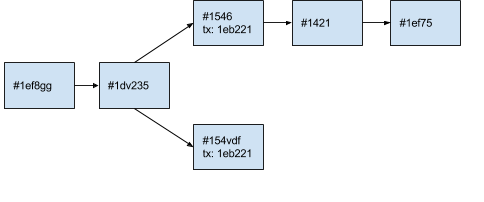
\includegraphics[scale=0.75]{grafiken/double_spending_sidechain.png}
	\caption{Double-spending über eine Sidechain (eigene Abbildung)}
	\label{double spending Attacke}
\end{figure}\todo{Grafik überarbeiten}

Bitcoin benötigt dafür jedoch einen Soft-Work um fähig zu sein, eine \ac{SPV} Prüfung auf der Sidechain durchzuführen. 
\subsubsection{Asymmetrischer two-way peg}
Sidechain Nutzer validieren die Parent-Chain komplett. Ein Litecoin-Nutzer hat also auch die Bitcoin-Blockchain gespeichert und kann alle Transaktionen validieren.
Umgekehrt wird SPV-Proof genutzt.
\subsubsection{Atomic Swaps}
Atomic Swaps sind ein weiterer Ansatz, um Werte zwischen zwei Parteien auf verschiedenen Chains auszutauschen. Dabei wird die gleiche Menge an Münzen, bzw. der gleiche Wert (bei unterschiedlichen Währungen) zw. zwei Parteien A und B ausgetauscht. Dazu benötigt A auf Chain 1 eine öffentliche Adresse pkA sowie ein Geheimnis a. B benötigt lediglich eine öffentliche Adresse. Der Austausch findet wie folgt statt:
\begin{enumerate}
	\item A initiiert Transaktion 1 (tx1) über eine Münze von pkA an einen Output O1, welcher entweder mit a und B's Signatur oder A's und B's Signatur geöffnet werden kann. Diese Transaktion wird noch nicht im Netzwerk veröffentlicht.
	\item A initiiert Transaktion 2 (tx2) in der nach einer locktime\footnote{Eine locktime ist eine bestimmte Zeit, die eine Transaktion nicht weiter ausgeführt werden kann} von 48 Stunden die Münze zurück an pkA überwiesen wird.
	\item B signiert tx2
	\item A kann nun tx1 im Netzwerk öffentlich machen
	\item B initiiert Transaktion 3 (tx3) über eine Münze von pkB an einen Output O2, welcher entweder mit a und B's Signatur oder A's und B's Signatur geöffnet werden kann. Diese Transaktion wird noch nicht im Netzwerk veröffentlicht.
	\item B initiiert Transaktion 4 (tx4) in der nach einer locktime von 24 die Münze zurück an pkB überwiesen wird.
	\item A signiert tx4
	\item B kann nun tx3 im Netzwerk öffentlich machen
	\item Nun kann A mit a auf die Münze in O2 zugreifen. Dies muss innerhalb von 24 Stunden geschehen, da sonst B automatisch Zugriff auf O2 erlangt.
	\item Durch den Zugriff auf O2 wird a veröffentlicht. Dadurch erlangt B Zugriff auf O1 und muss die Münze innerhalb von 48 Stunden überweisen, da sonst A automatisch Zugriff auf O1 erlangt.
\end{enumerate}\cite{TierNolan.2013}

Dadurch, dass - im Gegensatz zu two-way-pegged Sidechains - bei Atomic Swaps keine Münzen in einem Output \glqq eingefroren\grqq, sowie keine neuen Münzen auf der Sidechain erzeugt werden müssen, sondern sich lediglich der Besitzer ändert, können diese Swaps in etwa so schnell wie zwei normale Transaktionen durchgeführt werden. Er ist jedoch nur möglich, wenn eine Partei Interesse an Werten auf jeweils der anderen Chain hat und stellt daher keine Überweisung dar. \\
Im Gegensatz zu two-way-pegged Sidechains ist es jedoch möglich, einen Swap zw. zwei Währungen auszuführen, wenn sich beide Parteien auf einen bestimmten Wechselkurs einigen.
\subsubsection{Bewertung der Ansätze}
Das Koppeln einer Blockchain an die Bitcoin-Blockchain bringt verschiedene Vor- und Nachteile sowohl für die Parent-Chain als auch die Sidechain. 
\begin{enumerate}
	\item + Es entstehen Synergieeffekte. Eine erfolgreiche Sidechain profitiert von der Bitcoin Community und muss keine eigene Infrastruktur aufbauen. Dafür wächst die Bitcoin Community um die Anzahl der Sidechain-Nutzer.
	\item - Es ist nicht mehr über den Kurs der eigenen Crypto-Währung ersichtlich, wie erfolgreich die Sidechain ist. Die Marktkapitalisierung ist ein guter Indikator, wie stark ein neuer Ansatz akzeptiert wird. Dieser ist nur noch indirekt über die Entwicklung der Bitcoin Marktkapitalisierung sowie der auf die Sidechain übertragenen Münzen ableitbar.
	\item - Unausgereifte Sidechains stellen eine Gefahr für die Nutzer dar. Eine Übertragung von Werten zwischen verschiedenen Sidechains sollte einen Nutzer nicht interessieren müssen \todo{ordentlicher Satz}. Ist die Sidechain jedoch unsicher implementiert, oder wird sie nur von wenigen Minern geschützt, so ist sie anfällig für Angriffe. Durch den Diebstahl der Parent-Chain Währung würde dies stark den Ruf der Parent-Chain schädigen.
	\item + Nutzer müssen zur Verwendung der Zusatzfunktionen einer spezifischen Sidechain ihre Währung nicht umtauschen. Dies senkt die Eintrittshürde zur Verwendung.
\end{enumerate}

Sie sind jedoch ausgezeichnet dazu geeignet, um neue Features, Updates und Weiterentwicklungen zu testen, die bei Erfolg in die Parent-Chain übernommen werden. Dazu können auch ökonomische Experimente zählen. \\
Ein weiterer, vielversprechender Ansatz ist die Möglichkeit, mehrere Parallelwährungen auf einer Chain zu führen. \cite{Back.2014}[S.15f]
\subsection{Übertragung von Verträgen auf verschiedenen Chains}
Nicht nur die Übertragung von Werten zwischen verschiedenen Blockchains ist eine wichtige Funktionalität. Auch eine Kompatibilität und Ausführbarkeit von Vertragsbedingungen ist notwendig. Dies ist nur möglich, wenn entweder ein gemeinsamer Standard genutzt wird, oder verschiedene Blockchains jeweils den Interpreter einer Vertragssprache implementieren. Weiterhin müssen diese Blockchains per Definition Turing-Vollständig sein, da sie sonst keinen komplexen Programmcode interpretieren können \\
Rootstock behauptet, dass es Fähig ist, den Vertragscode von Ethereum zu kompilieren. \cite{Rootstock.2016}
\section{Architektur Turing-Vollständiger Blockchains am Beispiel Ethereum}
\section{Das Hyperledger Projekt/R3CEV \todo{wohl nicht mehr aktuell}}



\section{Coin-Arten}
Gedeckeltes inflationäres Modell --> Bitcoin
ungedeckeltes inflationäres Modell --> Ethereum, Dogecoin
Freicoin --> Bestimmte Geldmenge aber Geld wird regelmäßig von allen Kontenhaltern abgezogen und wieder dem Pool hinzugefügt
\section{Blockchain-as-a-Service}
